\XeTeXgenerateactualtext=1
\ifdefined\HANDOUT
  \documentclass[fontset=none,handout]{ctexbeamer}
\else
  \documentclass[fontset=none]{ctexbeamer}
\fi

\usepackage{%
  array,
  bookmark,
  booktabs,
  datetime2,
  fdulogo,
  fontawesome5,
  hologo,
  listings,
  multicol,
  qrcode,
  ragged2e,
  siunitx,
  xeCJKfntef,
  unicode-math}

\makeatletter

\@namedef{ver@beamerfontthememetropolis.sty}{9999/99/99}

% Beamer theme
\usetheme{Xiaoshan}
\usefonttheme{serif,professionalfonts}

% Beamer settings
\metroset{progressbar=none}
\setbeamerfont{title}{size=\huge, series=\bfseries}
\setbeamerfont*{subtitle}{size=\large, shape=\itshape}
\setbeamerfont{section title}{size=\Large, series=\bfseries}
\setbeamerfont{frametitle}{size=\large, series=\bfseries}
\setbeamerfont{caption}{size=\footnotesize, series=\bfseries}
\setbeamerfont{itemize/enumerate subbody}{size=\footnotesize}
\setbeamerfont{footnote}{size=\tiny}
\setbeamerfont{alerted text}{series=\bfseries}
\addtobeamertemplate{institute}{\raggedleft}{}
\setbeamertemplate{title}{%
  \raggedleft
  \linespread{1}%
  \inserttitle
  \hspace*{1.2cm}\par
  \vspace*{0.5em}}
\setbeamertemplate{subtitle}{%
  \raggedleft
  \insertsubtitle
  \hspace*{1.2cm}\par
  \vspace*{0.5em}}
\setbeamertemplate{title page}{%
  \begin{minipage}[b]{\textwidth}
    \usebeamertemplate*{title graphic}
    \usebeamertemplate*{title}
    \usebeamertemplate*{subtitle}
    \usebeamertemplate*{title separator}
    \usebeamertemplate*{author}
    \usebeamertemplate*{date}
    \usebeamertemplate*{institute}
    \vfill
  \end{minipage}}
\setbeamertemplate{title graphic}{%
  \vbox to 0pt {\smash{\raisebox{-128pt}{\inserttitlegraphic}}}%
  \nointerlineskip}
\setbeamertemplate{frame numbering}{\zhnumber[style=Financial]{\insertframenumber}}
\setbeamertemplate{caption}{\parbox{\textwidth}{\centering\insertcaption}\par}
\setbeamertemplate{bibliography item}[text]

% Colors
\colorlet{keyword}{松花绿}
\colorlet{comment}{漆黑!50}
\colorlet{texcs}{酡红}
\colorlet{emph1}{靛蓝}
\colorlet{emph2}{琥珀}
\colorlet{inline}{玄色}

% Fonts: basic
\setmainfont{LibertinusSerif}[
  Extension      = .otf,
  UprightFont    = *-Regular,
  BoldFont       = *-Bold,
  ItalicFont     = *-Italic,
  BoldItalicFont = *-BoldItalic,
  Scale          = 1.1]
\setmonofont{RobotoMono}[
  Extension      = .otf,
  UprightFont    = *-Regular,
  BoldFont       = *-Bold,
  ItalicFont     = *-Italic,
  BoldItalicFont = *-BoldItalic,
  Scale          = 0.92]
\setmathfont{LibertinusMath-Regular.otf}

\IfFontExistsTF{Source Han Serif SC}{
  \setCJKmainfont{Source Han Serif SC}[
    UprightFont    = * SemiBold,
    BoldFont       = * Heavy,
    ItalicFont     = * SemiBold,
    BoldItalicFont = * Heavy,
    CharacterWidth = Full]
}{
  \setCJKmainfont{Noto Serif CJK SC}[
    UprightFont    = * SemiBold,
    BoldFont       = * Black,
    ItalicFont     = * SemiBold,
    BoldItalicFont = * Black,
    CharacterWidth = Full]
}
\IfFontExistsTF{Source Han Serif SC}{
  \setCJKmonofont{Source Han Sans SC}[AutoFakeSlant]
}{
  \setCJKmonofont{Noto Sans CJK SC}[AutoFakeSlant]
}

% Fonts: TeX Live
\newfontfamily\Garamond{EBGaramond}[
  Extension      = .otf,
  UprightFont    = *-Regular,
  BoldFont       = *-Bold,
  ItalicFont     = *-Italic,
  BoldItalicFont = *-BoldItalic]
\newfontface\ArphicKai{gkai00mp.ttf}[AutoFakeBold=4, AutoFakeSlant]
\newfontface\Times{FreeSerif.otf}
\newfontface\Helvetica{FreeSans.otf}
\newfontface\Courier{FreeMono.otf}
\newfontface\Bodini{QTBodini.otf}
\newfontface\Futura{QTFuture.otf}
\newfontface\Optima{QTOptimum.otf}
\newfontface\Inconsolata{Inconsolatazi4-Regular.otf}
\newfontface\LibertinusKey{LibertinusKeyboard-Regular.otf}
\newfontface\LatinRomanV{lmroman5-regular.otf}
\newfontface\LatinRomanVI{lmroman6-regular.otf}
\newfontface\LatinRomanVII{lmroman7-regular.otf}
\newfontface\LatinRomanVIII{lmroman8-regular.otf}
\newfontface\LatinRomanIX{lmroman9-regular.otf}
\newfontface\LatinRomanX{lmroman10-regular.otf}
\newfontface\LatinRomanXII{lmroman12-regular.otf}
\newfontface\LatinRomanXVII{lmroman17-regular.otf}
\newCJKfontfamily\fangsong{FandolFang-Regular.otf}
\newCJKfontfamily\heiti{FandolHei-Regular.otf}
\newCJKfontfamily\kaishu{FandolKai-Regular.otf}

% Fonts: local
\newfontface\NotoDevanagari{NotoSerifDevanagari-Regular.otf}[Path=./fonts/, Script=Devanagari]
\newfontface\NotoArabic{NotoNaskhArabic-Regular.otf}[Path=./fonts/, Script=Arabic]
\newfontface\NotoEgyptian{NotoSansEgyptianHieroglyphs-Regular.otf}[Path=./fonts/]
\newfontface\Unifont{unifont-14.0.02.subset.ttf}[Path=./fonts/]
\newfontface\XKCD{xkcd-script.ttf}[Path=./fonts/, Ligatures=TeX]

% PDF bookmark
\apptocmd{\beamer@@frametitle}{%
  \only<1>{\expandafter\ifnum\insertcontinuationcount<2\relax
    \bookmark[page=\the\c@page,level=4]{#1}\fi}}{}{}

% Code listings
\lstdefinestyle{style@latex}{
  language     = [latex]TeX,
  alsoletter   = {*},
  keywordstyle = \bfseries\color{keyword},
  commentstyle = \itshape\color{comment},
  texcsstyle   = *\color{texcs},
  emphstyle    = [1]\itshape\color{emph1},
  emphstyle    = [2]\color{emph2}
}
\lstdefinestyle{style@inline}{
  basicstyle   = \ttfamily\color{inline},
  keepspaces   = true
}
\lstnewenvironment{texcode}[1][]{\lstset{
  style        = style@latex,
  basicstyle   = \footnotesize\ttfamily,
  gobble       = 2,
  morekeywords = {\documentclass,\usepackage,\begin,\end},#1}}{}
\lstMakeShortInline[style=style@inline]|

% Hack
% Use small caps for LaTeX symbol
\DeclareRobustCommand{\LaTeX}{%
  L\kern-.3em%
  \raisebox{.2em}{\textsc{a}}\kern-.14em%
  \TeX}
% Compatibility with unicode-math
\DeclareRobustCommand{\LaTeXe}{%
  \LaTeX\kern.15em2%
  \hbox{%
    \if b\expandafter\@car\f@series\@nil
      $_{\textstyle\symbf{\varepsilon}}$%
    \else
      $_{\textstyle\varepsilon}$%
    \fi}}
% PoZheHao, see https://github.com/CTeX-org/ctex-kit/issues/382
\ExplSyntaxOn
\xeCJK_new_class:n { PoZheHao }
\__xeCJK_save_CJK_class:n { PoZheHao }
\xeCJK_declare_char_class:nn { PoZheHao } { "2014 }
\seq_map_inline:Nn \g__xeCJK_class_seq
  {
    \str_if_eq:nnF {#1} { PoZheHao }
      {
        \xeCJK_copy_inter_class_toks:nnnn { PoZheHao } {#1} { FullRight } {#1}
        \xeCJK_copy_inter_class_toks:nnnn {#1} { PoZheHao } {#1} { FullRight }
      }
  }
\ExplSyntaxOff

% Commands
\newcommand{\link}[1]{\href{#1}{\faLink}}
\newcommand{\CASE}[1]{{\addfontfeatures{Letters=Uppercase}#1}}
\newcommand{\jatext}[1]{{\addCJKfontfeatures{Language=Japanese}#1}}
\newcommand{\zhparen}[1]{(\raisebox{0.1ex}{#1})}
\newcommand{\enparen}[1]{\CASE{(}#1\CASE{)}}
\newcommand{\pkg}[1]{\texttt{#1}}
\newcommand{\usv}[1]{\texttt{U+#1}}
\newcommand{\kbd}[1]{{\LibertinusKey#1}}
\newcommand{\nonumberfootnote}[2][]{%
  \let\thefootnote\relax
  \footnotetext#1{#2}}
\renewcommand{\footnoterule}{}

\newcommand{\XeTeX}{\hologo{XeTeX}}
\newcommand{\pdfTeX}{\hologo{pdfTeX}}
\newcommand{\LuaTeX}{\hologo{LuaTeX}}
\newcommand{\XeLaTeX}{\hologo{Xe}\kern-.13em\LaTeX{}}
\newcommand{\pdfLaTeX}{pdf\LaTeX{}}
\newcommand{\LuaLaTeX}{Lua\LaTeX{}}
\newcommand{\BibTeX}{\hologo{BibTeX}}

\makeatother

% Information
\title{现代 \LaTeX{} 入门讲座}
\subtitle{Modern \LaTeX{} in a Nutshell}
\author{曾祥东}
\institute{复旦大学\quad 物理系}
\date{\zhtoday}
\titlegraphic{\qrcode[hyperlink, height=1.6cm]{https://github.com/stone-zeng/latex-talk}}

\begin{document}

\maketitle

\begin{frame}[standout]
  \large\XKCD
  ``Your paper makes no goddamn sense, \\
  but it's the most beautiful thing \\
  \XeTeXglyph\XeTeXglyphindex"I_hyphen_p_r_o_n_o_u_n"\relax\
  have ever laid eyes on.''

  \small
  \hfill From r/ProgrammerHumor
  \href{https://www.reddit.com/r/ProgrammerHumor/comments/2jf7yl}{\faRedditAlien}
\end{frame}

\section{介绍}

\begin{frame}{历史回眸}
\begin{columns}
\begin{column}{0.45\textwidth}
  \begin{figure}
    \centering
    \includegraphics[height=3.2cm]{images/knuth-2018.jpg}
    \caption{高德纳(Donald~E. Knuth) \\ \TeX}
  \end{figure}
\end{column}
\begin{column}{0.45\textwidth}
  \begin{figure}
    \centering
    \includegraphics[height=3.2cm]{images/lamport-2018.jpg}
    \caption{Leslie Lamport \\ \LaTeX}
  \end{figure}
\end{column}
\end{columns}
\nonumberfootnote{图片来源:
  \link{https://www-cs-faculty.stanford.edu/~knuth/graphics.html}
  \link{https://aperiodical.com/2018/09/hlf-blogs-leslie-lamport-thinks-your-code-is-bad}}
\end{frame}

\begin{frame}{\LaTeX{} 是什么?}
\pause
\begin{itemize}
  \item<+-> 发音:

    \begin{itemize}
      \item /ˈlɑːtɛx/ or /ˈleɪtɛx/ or whatever you like
    \end{itemize}

  \item<+-> 打公式方便?

    \begin{itemize}
      \item 「复杂公式输入哪家强,当然首选 \LaTeX{} 帮忙」
    \end{itemize}

  \item<+-> 写论文神器?

    \begin{itemize}
      \item 「想要轻松给论文排版,当然少不了 \LaTeX{} 啦」
    \end{itemize}

  \item<+-> 不想做宏编程的标记语言不是好的排版引擎?

    \begin{itemize}
      \item {\tiny
        \LaTeX{} is a high-quality typesetting system; it includes features
        designed for the production of technical and scientific documentation.
        \LaTeX{} is the \textit{de facto} standard for the communication and
        publication of scientific documents. \LaTeX{} is available as free
        software. \link{https://www.latex-project.org}}
    \end{itemize}
\end{itemize}
\end{frame}

\begin{frame}[fragile]
\frametitle{\LaTeX{} 是什么?\mbox{}——\mbox{}What you \emph{think} is what you get!}
\begin{columns}
\begin{column}{0.5\textwidth}
  \begin{texcode}[basicstyle=\tiny\ttfamily, moretexcs={\maketitle},
    emph={[1]equation,itemize,document}, emph={[2]article,amsmath,graphicx}]
  \documentclass{article}
  \usepackage{amsmath,graphicx}
  \title{Normal distribution}
  \author{Wikipedia, the free encyclopedia}

  \begin{document}
  \maketitle
  \section{Introduction}
  % 省略一些内容……
  The probability density of the normal
  distribution is
  \begin{equation}
    f(x|\mu, \sigma)
    = \frac{1}{\sqrt{2\pi\sigma^2}}
      e^{-\frac{(x-\mu)^2}{2\sigma^2}}
  \end{equation}
  where
  \begin{itemize}
    \item $\mu$ is the mean of the distribution
    \item $\sigma$ is the standard deviation
  \end{itemize}
  \end{document}
  \end{texcode}
\end{column}
\pause
\begin{column}{0.42\textwidth}
  \begin{figure}
    \centering
    \vspace{-0.8cm}
    \includegraphics[width=\textwidth, trim={2cm 2cm 2cm 2cm}, clip]%
      {examples/normal-dist/normal-dist.pdf}
  \end{figure}
\end{column}
\end{columns}
\nonumberfootnote{来源:Wikipedia \link{https://en.wikipedia.org/wiki/Normal_distribution}}
\end{frame}

\begin{frame}{基本原则}
\begin{itemize}
  \item<+-> 排版 vs 文字处理

    \begin{itemize}
      \item 《别把 \LaTeX{} 当 Word 用》
    \end{itemize}

  \item<+-> 遵循业\zhparen{xué}界\zhparen{xiào}规范

    \begin{itemize}
      \item 《管教务处 or 研究生院 or 物理系叫爸爸》
    \end{itemize}

  \item<+-> 追求良好的阅读体验\zhparen{readability}
  \item<+-> 内容与格式分离
  \item<+-> \alert{内容永远比格式重要!}

    \begin{itemize}
      \item \emph{Typography exists to honor content.} ---R. Bringhurst
    \end{itemize}
\end{itemize}
\end{frame}

\section{安装}

\begin{frame}{不想安装?}
\begin{itemize}
  \item 云端服务可能更好用
  \item 免去安装、升级等一系列烦恼,可以多人协作
  \item 国际版:\href{https://www.sharelatex.com}{\textcolor{酡红}{ShareLaTeX}} 和
        \href{https://www.overleaf.com}{\textcolor{松花绿}{Overleaf}}(现已合并)

    \begin{itemize}
      \item 模板丰富
      \item 用户支持很好(支持团队中有华人)
      \item 注册及使用可能遇到网络问题
    \end{itemize}

  \item 国内版:TeXPage \link{https://www.texpage.com}

    \begin{itemize}
      \item 网络限制较少
      \item 支持更多的中文字体
      \item 不够成熟稳定
      \item 免费账号项目数量受限
    \end{itemize}
\end{itemize}
\end{frame}

\begin{frame}{选择发行版}
\begin{itemize}
  \item \TeX{} 发行版\zhparen{distribution}

    \begin{itemize}
      \item 引擎、宏包、字体、文档的综合体
      \item 类比 Visual Studio
      \item \TeX{} Live、Mac\TeX{}、MiK\TeX{} 等
    \end{itemize} \pause

  \item \TeX{} Live \link{https://www.tug.org/texlive}

    \begin{itemize}
      \item 官方维护,首选,跨平台
      \item Mac\TeX{} ≈ macOS 下的 \TeX{} Live
      \item 缺点:完整版体积大\zhparen{3GB+}、每年需重装
    \end{itemize}

  \item MiK\TeX{} \link{https://miktex.org}

    \begin{itemize}
      \item 由 Christian Schenk 维护(是个狠人)
      \item 宏包随用随装
      \item 缺点:部分细节与 \TeX{} Live 不兼容、网络问题
    \end{itemize} \pause

  \item \alert{不要安装 \CTeX{} 套装!}

    \begin{itemize}
      \item \alert{存在严重 bug,并且完全过时}
    \end{itemize}
\end{itemize}
\end{frame}

\begin{frame}{下载}
\begin{itemize}
  \item 选择国内 CTAN 镜像

    \begin{itemize}
      \item 清华大学开源软件镜像站 \link{https://mirrors.tuna.tsinghua.edu.cn}
      \item 上海交通大学软件源镜像服务 \link{https://mirrors.sjtug.sjtu.edu.cn}
      \item 中国科学技术大学开源软件镜像 \link{https://mirrors.ustc.edu.cn} \pause
      \item 复旦大学……
    \end{itemize} \pause

  \item 建议使用 ISO 镜像离线安装
  \item 在线安装要求网络稳定
\end{itemize}
\end{frame}

\begin{frame}{安装流程}
\begin{itemize}
  \item 新手建议安装完整版 \TeX{} Live 或 Mac\TeX{}

    \begin{itemize}
      \item 完整版可避免后续维护烦恼
      \item 一路点击「下一步」
      \item 保持耐心,做好重装的打算
    \end{itemize} \pause

  \item Linux specials

    \begin{itemize}
      \item 软件源更新较慢,可以考虑 Vanilla \TeX{} Live
      \item GUI 安装界面需要 \pkg{perl-tk} 等
      \item 环境变量、\pkg{fontconfig}、dummy package 配置
    \end{itemize}

  \item macOS specials

    \begin{itemize}
      \item 推荐 Homebrew \href{https://brew.sh/}{\faBeer}
    \end{itemize}

  \item 手把手的教程:\link{https://github.com/OsbertWang/install-latex-guide-zh-cn}
\end{itemize}
\end{frame}

\begin{frame}[fragile]
\frametitle{神圣的战争——选择编辑器}
\begin{itemize}
  \item<+-> 专用型

    \begin{itemize}
      \item TeXworks:\TeX{} Live 自带 \faWindows{} \faApple{} \faLinux{}
      \item TeXstudio:功能丰富,对新手友好 \faWindows{} \faApple{} \faLinux{}
      \item TeXShop:Mac\TeX{} 自带 \faApple{}
      \item WinEdt:功能丰富,收费 \faWindows{}
    \end{itemize}

  \item<+-> 通用型

    \begin{itemize}
      \item Visual Studio Code:配合 LaTeX Workshop 插件
      \item Sublime Text:需要收费
      \item Vim:|q|、|q!|、|wq|、|wq!|
    \end{itemize}

  \item<+-> 编辑器对比:\link{https://tex.stackexchange.com/q/339}
                        \link{https://en.wikipedia.org/wiki/Comparison_of_TeX_editors}
                        \link{https://www.zhihu.com/question/19954023}
\end{itemize}
\end{frame}

\section{开始之前……}

\begin{frame}[fragile]
\frametitle{命令行基础}
\begin{itemize}
  \item 打开终端

    \begin{itemize}
      \item \faWindows{}:右键开始菜单、空白处 \kbd{Shift} + 右键、\kbd{Windows} + \kbd{R} \& |cmd|
      \item \faLinux{}:\kbd{Ctrl} + \kbd{Alt} + \kbd{T}
      \item \faApple{}:\kbd{⌘} + \kbd{Space} 搜索 Terminal、可在 Finder 中添加服务
    \end{itemize}

  \item 基本命令:

    \begin{itemize}
      \item |cd|、|ls/dir|、|rm/del|、|clear/cls|
      \item 选项:|-h|、|--help|、|/?|
    \end{itemize}

  \item 其他:

    \begin{itemize}
      \item 复制粘贴:\kbd{Ctrl}/\kbd{Shift} + \kbd{Ins}、\kbd{Ctrl}/\kbd{⌘} + \kbd{C}/\kbd{V}、
      \item 路径连接符:斜线(|/|)或反斜线(|\|)
      \item 换行符:LF(|\n|)或 CRLF(|\r\n|)
      \item 结束进程:\kbd{Ctrl} + \kbd{C}
    \end{itemize} \pause

  \item \alert{尽量不要用中文;避免空格、特殊符号}
\end{itemize}
\end{frame}

\begin{frame}{编码}
关于 \LaTeX{} 源文件的编码,我们给出如下结论:\pause
\begin{alertblock}{编码定理}
  \vspace{0cm}
  一般地,在任何场合使用(不带 BOM 的) \alert{UTF\CASE{-}8} 编码均是最优选择.
\end{alertblock} \pause
此定理的证明留做习题.
\end{frame}

\section{填写内容}

\begin{frame}[fragile]
\frametitle{Hello world!}
\begin{texcode}[basicstyle=\small\ttfamily, xleftmargin=1.2cm,
    emph={[1]document}, emph={[2]article}]
  % 用 pdfLaTeX、XeLaTeX 或 LuaLaTeX 编译
  \documentclass{article}
  \begin{document}
  Hello world!
  \end{document}
\end{texcode}
\pause
\begin{texcode}[basicstyle=\small\ttfamily, xleftmargin=1.2cm,
    emph={[1]document}, emph={[2]ctexart}]
  % 用 XeLaTeX 或 LuaLaTeX 编译
  \documentclass{ctexart}
  \begin{document}
  你好,世界!
  \end{document}
  \end{texcode}
\end{frame}

\begin{frame}[fragile]
\frametitle{引擎与格式}
\begin{itemize}
  \item<+-> \textbf{引擎}:\TeX{} 的实现

    \begin{itemize}
      \item \pdfTeX{}:直接生成 PDF,支持 micro-typography
      \item \XeTeX{}:支持 Unicode、OpenType 与复杂文字编排(CTL)
      \item \LuaTeX{}:支持 Unicode、OpenType,内联 Lua
      \item (u)p\TeX{}:日本方面推动,生成 |.dvi|,(支持 Unicode)
      \item Ap\TeX{}:底层 CJK 支持,内联 Ruby,Color Emoji(手动斜眼笑)
    \end{itemize}

  \item<+-> \textbf{格式}:\TeX{} 的语言扩展(命令封装)

    \begin{itemize}
      \item plain \TeX{}:Knuth 同志专用
      \item \LaTeX{}:排版科技类文章的事实\zhparen{\textit{de facto}}标准
      \item Con\TeX t:基于 \LuaTeX{} 实现,优雅、易用(吗?)
    \end{itemize}

  \item<+-> \textbf{程序}:引擎 + dump 之后的格式代码

    \begin{itemize}
      \item \alert{英文文章:\pdfLaTeX{}、\XeLaTeX{} 或 \LuaLaTeX{}}
      \item \alert{中文文章:\XeLaTeX{} 或 \LuaLaTeX{}}
    \end{itemize}
\end{itemize}
\end{frame}

\begin{frame}[fragile]
\frametitle{编译}
\begin{itemize}
  \item 现代 \TeX{} 引擎均可直接生成 PDF \pause
  \item 命令行

    \begin{itemize}
      \item |pdflatex|/|xelatex|/|lualatex| + |<文件名>[.tex]|
      \item 多次编译:读取并排版中间文件 \pause
      \item 推荐 \pkg{latexmk}:|latexmk [<选项>] [<文件名>]|
    \end{itemize} \pause

  \item 编辑器

    \begin{itemize}
      \item 按钮的背后仍然是命令
      \item |PATH| 环境变量:确定可执行文件的位置
      \item VS Code:配置 |tools| 和 |recipes|
    \end{itemize}
\end{itemize}
\end{frame}

\begin{frame}[fragile]
\frametitle{语法}
\begin{itemize}
  \item 注释以 |%| 开头,忽略其后所有内容
  \item 命令以 |\| 开头,区分大小写

    \begin{itemize}
      \item |\foo{arg}|:必选参数放在 |{...}| 中
      \item |\foo[bar]{arg}|:可选参数放在 |[...]|
    \end{itemize}

  \item 环境

    \begin{texcode}[gobble=4, emph={[1]env}]
      \begin{env}
        ...
      \end{env}
    \end{texcode}

  \item 特殊符号需要转义:|\%|、|\$|、|\&|、|\textbackslash| 等
  \item 连续多个空格 = 单个空格 = 单个换行符 \pause
  \item \TeX{}/\LaTeX{} 的语法可以修改
\end{itemize}
\end{frame}

\begin{frame}[fragile]
\frametitle{文件结构}
\begin{texcode}[basicstyle=\scriptsize\ttfamily, moretexcs={\keyword,\boldsymbol},
    emph={[1]document}, emph={[2]article,amsmath}]
  % 用 UTF-8 编码,命名为 xxx.tex
  \documentclass{article}                     % 指明文档类型:文章
  % 导言区:设置文档样式
  \usepackage{amsmath}                        % 调用宏包,实现各种功能
  \newcommand{\keyword}[1]{\textbf{#1}}       % 自定义命令

  \begin{document}
  % 正文:套用格式
  In quantum mechanics, the \keyword{Schr\"odinger equation} is a
  mathematical equation that describes the changes over time of a
  physical system in which quantum effects, such as \keyword{wave--%
  particle duality}, are significant.

  % 上面的空行表示分段
  In classical mechanics, Newton's second law
  ($\boldsymbol{F}=m\boldsymbol{a}$) is used to make a\ldots{}

  Time-dependent Schrödinger equation can be written as  % ö 也能直接用
  \[ i\hbar \frac{d}{dt} |\Psi(t)\rangle = \hat{H} |\Psi(t)\rangle. \]
  \end{document}
\end{texcode}
\vspace{-0.6cm}
\end{frame}

\begin{frame}{Schrödinger equation}
In quantum mechanics, the \textbf{Schr\"odinger equation} is a
mathematical equation that describes the changes over time of a
physical system in which quantum effects, such as \textbf{wave--%
particle duality}, are significant.

In classical mechanics, Newton's second law
($\mathbfit{F}=m\mathbfit{a}$) is used to make a\ldots{}

Time-dependent Schrödinger equation can be written as
\[ i\hbar \frac{d}{dt} \vert\Psi(t)\rangle = \hat{H} \, \vert\Psi(t)\rangle. \]
\end{frame}

\begin{frame}[fragile]
\frametitle{谋篇布局}
\begin{itemize}
  \item 文档部件

    \begin{itemize}
      \item 标题:|\title|、|\author|、|\date| $\to$ |\maketitle|
      \item 摘要:|abstract| 环境
      \item 目录:|\tableofcontents|
      \item 章节:|\chapter|、|\section|、|\subsection| 等
      \item 文献:|\bibliography|
    \end{itemize}

  \item 文档划分

    \begin{itemize}
      \item 凤头猪肚豹尾:|\frontmatter|、|\mainmatter|、|\backmatter|
      \item 分文件编译:|\include|、|\input|
    \end{itemize}
\end{itemize}
\end{frame}

\begin{frame}[fragile]
\frametitle{文本标记(一)}
\begin{itemize}
  \item 加粗:|{\bfseries ...}| 或 |\textbf{...}|
  \item 倾斜:|{\itshape ...}| 或 |\textit{...}|
  \item 字号:|\tiny|、|\small|、|\large|、|\Large| 等
  \item 换行:|\\|
  \item 缩进:|\indent|
  \item 居中:|\centering| 或 |center| 环境
\end{itemize}
\end{frame}

\begin{frame}[standout]
  \huge \textbf{请忘记上一页}
\end{frame}

\begin{frame}[fragile]
\frametitle{文本标记(二)}
\begin{itemize}
  \item 为什么要有不同的标记?\pause\mbox{}——表达不同的\alert{语义} \pause
  \item |\textbf| 这样的命令是否表达语义? \pause
  \item 再提一遍基本原则:\alert{内容与格式分离} \pause
  \item 正确(或曰:合理)的做法

    \begin{itemize}
      \item 强调文字(意大利体):|\emph{...}|
      \item 摘要(居中,小字号,带有标题):|abstract| 环境
      \item 引用(左右边距较大):|quote| 或 |quotation| 环境
      \item 自定义新的命令、环境
    \end{itemize} \pause

  \item 报告,我想偷懒!
  \item 报告,我听说了 Tailwind CSS \link{https://tailwindcss.com}!
\end{itemize}
\end{frame}

\begin{frame}[fragile]
\frametitle{常用环境:列表与枚举}
\begin{columns}
\begin{column}{0.54\textwidth}
  \begin{texcode}[gobble=4, emph={[1]enumerate,itemize}]
    \begin{enumerate}
      \item Frontend
        \begin{itemize}
          \item React
          \item Vue.js
          \item Svelte
        \end{itemize}
      \item Backend
        \begin{description}
          \item[PHP] Laravel
          \item[JavaScript] Express
          \item[Python] Django
        \end{description}
    \end{enumerate}
  \end{texcode}
\end{column}
\pause
\begin{column}{0.38\textwidth}
  \begin{enumerate}
    \item Frontend
      \begin{itemize}
        \item React
        \item Vue.js
        \item Svelte
      \end{itemize}
    \item Backend \par
        \vspace{0.5ex}\small
        \textbf{PHP}\enspace Laravel \\
        \textbf{JavaScript}\enspace Express \\
        \textbf{Python}\enspace Django
  \end{enumerate}
\end{column}
\end{columns}
\end{frame}

\begin{frame}[fragile]
\frametitle{常用环境:图片}
\begin{columns}
\begin{column}{0.64\textwidth}
  \begin{texcode}[gobble=4, moretexcs={\graphicspath,\includegraphics},
      emph={[1]figure}, emph={[2]graphicx}]
    % 不是 graphics
    \usepackage{graphicx}
    % 可以统一指定图片路径
    \graphicspath{{./images/}}

    \begin{figure}
      \centering
      % 可指定宽度、高度等选项
      % 图片后缀名可省略,但建议保留
      \includegraphics[...]{fudan-logo.pdf}
      \caption{Logo of Fudan University}
      \label{fig:fudan-logo}
    \end{figure}
  \end{texcode}
\end{column}
\pause
\begin{column}{0.28\textwidth}
  \begin{figure}
    \centering
    \fduemblem+[x=0.1pt, y=0.1pt, color=FudanBlue]
    \caption{\textcolor{keyword}{Figure \thefigure:} Logo of Fudan University}
    \label{fig:fudan-logo_}  % Avoid duplicate labels warning
  \end{figure}
\end{column}
\end{columns}
\end{frame}

\begin{frame}[fragile]
\frametitle{常用环境:表格}
\begin{columns}
\begin{column}{0.62\textwidth}
  \begin{texcode}[gobble=4, moretexcs={\toprule,\midrule,\bottomrule},
      emph={[1]table,tabular}, emph={[2]booktabs}]
    \usepackage{booktabs} % 三线表
    \begin{table}
      \caption{Population Census of China}
      \label{tab:china-population}
      % 列格式:c 居中,l 左对齐,r 右对齐
      \begin{tabular}{cc}
        \toprule
          Year & Population \\
        \midrule
          1953 &  6.0 \\
          ...
          2020 & 14.1 \\
        \bottomrule
      \end{tabular}
    \end{table}
  \end{texcode}
\end{column}
\pause
\begin{column}{0.3\textwidth}
  \begin{table}
    \caption{\textcolor{keyword}{Table \thetable:} Population Census of China}
    \label{tab:china-population_}
    \footnotesize
    \begin{tabular}{cc}
      \toprule
        Year & Population \\
      \midrule
        1953 &  6.0 \\
        1964 &  6.9 \\
        1982 & 10.1 \\
        1990 & 11.3 \\
        2000 & 12.7 \\
        2010 & 13.4 \\
        2020 & 14.1 \\
      \bottomrule
    \end{tabular}
  \end{table}
\end{column}
\end{columns}
\end{frame}

\begin{frame}[fragile]
\frametitle{常用环境:定理}
\begin{columns}
\begin{column}{0.6\textwidth}
  \begin{texcode}[gobble=4, moredelim={[is][emphstyle]{!}{!}}, moretexcs={\newtheorem*},
      emph={[2]amsthm}]
    \usepackage{amsthm}
    % 需要预先定义
    \newtheorem{theorem}{Theorem}
    \newtheorem*{remark}{Remark} % 不编号

    \begin{!theorem!}[Fermat]
      $a^n+b^n=c^n$ has no positive...
    \end{!theorem!}
    \begin{!proof!}
      % 证明后面会有 QED 符号
      It's obvious.
    \end{!proof!}
    \begin{!remark!}
      The cases $n=1$ and $n=2$...
    \end{!remark!}
  \end{texcode}
\end{column}
\pause
\begin{column}{0.32\textwidth}
  \footnotesize\RaggedRight
  \setlength{\parskip}{0.5em}
  \setlength{\parindent}{0pt}

  \textbf{Theorem 1} (Fermat). \textit{$a^n+b^n=c^n$ has no positive integer solutions
    for $x$, $y$ and $z$ when $n$ is greater than 2.}

  \textit{Proof.} It's obvious. \hfill $\mdlgwhtsquare$

  \textbf{Remark.} \textit{The cases $n=1$ and $n=2$ have been known since antiquity
    to have infinitely many solutions.}
\end{column}
\end{columns}
\end{frame}

\begin{frame}[fragile]
\frametitle{浮动体与交叉引用}
\begin{itemize}
  \item<+-> 浮动体机制

    \begin{itemize}
      \item |figure| 和 |table| 环境,标题使用 |\caption| 命令
      \item 位置控制:|\begin{figure}[htb]|
      \item 希望浮动体不要乱跑:「这是病,得治」
            \link{https://liam.page/2017/03/11/floats-in-LaTeX-basic}
      \item 文本为主,图、表为辅
      \item 避免「见上图」、「见下表」
      \item 建议写完全文之后统一调整
    \end{itemize}

  \item<+-> 以标签控制交叉引用

    \begin{itemize}
      \item 被引处:|\label|
      \item 引用处:|\ref|、|\eqref|、|\autoref| 等(如图~\textcolor{emph1}{\ref{fig:fudan-logo_}}、
            表~\textcolor{emph1}{\ref{tab:china-population_}})
      \item 用有意义的标签:|\label{eq:euler-lagrange-eq}|
      \item \pkg{hyperref}:添加超链接、电子书签等
      \item 需多次编译——推荐 \pkg{latexmk}
    \end{itemize}
\end{itemize}
\end{frame}

\begin{frame}[fragile]
\frametitle{如何在论文中画出漂亮的插图?}
\begin{itemize}
  \item<+-> 外部插入

    \begin{itemize}
      \item Mathematica、MATLAB
      \item PowerPoint、Visio、Adobe Illustrator、Inkscape、Figma 等
      \item Python \texttt{Matplotlib}、\texttt{Plots.jl}、R、Plotly 等
      \item draw.io \link{https://www.draw.io}、
            Mathcha \link{https://www.mathcha.io}、
            ProcessOn \link{https://www.processon.com} 等网站
    \end{itemize}

  \item<+-> \TeX{} 内联

    \begin{itemize}
      \item Asymptote
      \item \alert{\pkg{pgf}/\pkg{TikZ}、\pkg{pgfplots}}
    \end{itemize}

  \item<+-> 插图格式

    \begin{itemize}
      \item 矢量图:|.pdf|
      \item 位图:|.jpg| 或 |.png|
      \item \alert{不再推荐 \texttt{.eps}}
      \item 不(完全)支持 |.svg|、|.bmp|
    \end{itemize}

  \item<+-> 参考:\link{https://www.zhihu.com/question/21664179}
                  \link{https://tex.stackexchange.com/q/158668}
                  \link{https://tex.stackexchange.com/q/72930}
\end{itemize}
\end{frame}

\begin{frame}[fragile]
\frametitle{文献}
\begin{itemize}
  \item 建议自动生成\pause (你只有三篇参考文献?)\pause
  \item |.bib| 数据库(条目会包含 key,用于引用)

    \begin{itemize}
      \item Google Scholar 复制,Zotero、Jabref 等生成
      \item 注意特殊符号、公式等常常需要人工检查
    \end{itemize} \pause

  \item 传统方法:\BibTeX{} 后端

    \begin{itemize}
      \item 指定样式:|\bibliographystyle{<style>}|(导言区)
      \item 标记引用:|\cite{<key>}|
      \item 插入参考文献:|\bibliography{<bib 文件>}|
      \item 更多文献、引用样式:\pkg{natbib} 宏包
      \item 国家标准 GB/T 7714--2015
            \link{https://www.gb688.cn/bzgk/gb/newGbInfo?hcno=7FA63E9BBA56E60471AEDAEBDE44B14C}
            \link{https://github.com/Haixing-Hu/GBT7714-2005-BibTeX-Style/files/153951/GBT.7714-2015.pdf}:
            \alert{\pkg{gbt7714} 宏包}
    \end{itemize} \pause

  \item 现代方法:\pkg{biber} 后端 + \pkg{biblatex} 宏包

    \begin{itemize}
      \item 国家标准:\pkg{biblatex-gb7714-2015} 宏包
    \end{itemize} \pause

  \item 需多次编译——再次推荐 \pkg{latexmk}
\end{itemize}
\end{frame}

\begin{frame}[standout]
  \begingroup
    \fontsize{72}{84}\selectfont
    \textbf{𰻝}
  \endgroup \\[2ex]
  \footnotesize \usv{30EDE}
\end{frame}

\begin{frame}{中文支持}
\begin{columns}
\begin{column}{0.66\textwidth}
  \begin{itemize}
    \item 中文有什么特殊?\pause

      \begin{itemize}
        % Unicode 15.1
        % https://twitter.com/ken_lunde/status/1651215492840067072
        \item 汉字太多\zhparen{97,661+} \pause
        \item 横排 + 直排、标点禁则、行间注 \link{https://www.w3.org/TR/clreq} \pause
        \item \jatext{にほんご}、
              {\NotoDevanagari देवनागरी}、
              {\NotoArabic العَرَبِيَّة}、
              {\NotoEgyptian 𓅡𓎡𓅱𓀀𓏪}
      \end{itemize} \pause

    \item 已淘汰:

      \begin{itemize}
        \item CCT 系统、\pkg{CJK} 宏包(裸用)
        \item \CTeX{} 套装
      \end{itemize} \pause

    \item 目前推荐手段:

      \begin{itemize}
        \item \alert{\pkg{ctex} 宏集}(此 \pkg{ctex} 非彼 \CTeX{})
        \item \XeLaTeX{} 编译
      \end{itemize} \pause

    \item 可以用,不推荐:

      \begin{itemize}
        \item \pkg{xeCJK} 宏包(裸用)
        \item \pkg{ctex} 宏集 + 其他引擎编译
      \end{itemize}
  \end{itemize}
\end{column} \pause
\begin{column}{0.32\textwidth}
  \tiny
  \begin{tabular}{cc}
    \includegraphics[width=24pt]{images/leoliu.png}        &
    \includegraphics[width=24pt]{images/qinglee.jpg}       \\
    刘海洋 & 李清 \\[2ex]
    \includegraphics[width=24pt]{images/wulingyun.jpg}     &
    \includegraphics[width=24pt]{images/jjgod.jpg}         \\
    吴凌云 & 江疆 \\[2ex]
    \includegraphics[width=24pt]{images/li-a-ling.jpg}     &
    \includegraphics[width=24pt]{images/liam-huang.jpg}    \\
    马起园 & 黄晨成 \\[2ex]
    \includegraphics[width=24pt]{images/louisstuart96.jpg} &
    \includegraphics[width=24pt]{images/zepinglee.jpg}     \\
    鲁尚文 & 李泽平 \\[2ex]
    \includegraphics[width=24pt]{images/muzimuzhi.jpg}     &
    \includegraphics[width=24pt]{images/ruixi-zhang.png}   \\
    周宇恺 & 张瑞熹
  \end{tabular}
  \vspace{-0.6cm}
\end{column}
\end{columns}
\nonumberfootnote[<8->]{图片来源:GitHub、Twitter、知乎}
\end{frame}

\begin{frame}[fragile]
\frametitle{幻灯片}
\begin{itemize}
  \item<+-> 基本框架

    \begin{itemize}
      \item \pkg{beamer} 或 \pkg{ctexbeamer} 文档类
      \item 页面由 |frame| 环境组织
      \item 文本内容:建议使用 |itemize| 和 |enumerate|
      \item 图表:不再浮动,不建议使用交叉引用
      \item 定理及强调:|theorem|、|proof|、|block| 等
      \item 分栏:|columns| + |column| 环境
    \end{itemize}

  \item<+-> 主题与样式

    \begin{itemize}
      \item |\usetheme|、\lstinline[style=style@inline]+\use[font|color|inner|outer]theme+
      \item 更现代的主题:|metropolis|
      \item 使用「默认」字体:|\usefonttheme{serif}|
    \end{itemize}

  \item<+-> 动画(覆盖)

    \begin{itemize}
      \item |\pause| 命令
      \item |\onslide<1>|、|\item<1->| 等
    \end{itemize}
\end{itemize}
\end{frame}

\section{使用模板}

\begin{frame}[fragile]
\frametitle{模板}
\begin{itemize}
  \item<+-> 是什么?

    \begin{itemize}
      \item 设计好的格式框架
      \item 专注于内容:\alert{不必追求与期刊排版完全一致}
      \item Word 中的样式:「学好 \LaTeX{} 可以更科学地使用 Word」
    \end{itemize}

  \item<+-> 有哪些?

    \begin{itemize}
      \item 期刊:\pkg{revtex}、\pkg{elsarticle}、\pkg{IEEEtran}……
      \item 学位论文:\pkg{thuthesis}、\pkg{ustcthesis}、\pkg{SJTUThesis}……
    \end{itemize}

  \item<+-> 怎么用?

    \begin{itemize}
      \item |\documentclass{...}|,配置参数,照常编写
      \item 可能与 \LaTeX{} 通常用法不同:\alert{看文档,看文档,看文档}
    \end{itemize}

  \item<+-> 去哪里找?

    \begin{itemize}
      \item CTAN \link{https://ctan.org} 或 GitHub \href{https://github.com}{\faGithub}
      \item 期刊官网
      \item 「湿兄用 U 盘 or 微信传给你的模板几乎一定是过时的」
    \end{itemize}
\end{itemize}
\end{frame}

\begin{frame}[fragile]
\frametitle{\pkg{revtex}}
\begin{itemize}
  \item<+-> 获取

    \begin{itemize}
      \item APS 官网 \link{https://journals.aps.org/revtex}
      \item \TeX{} Live 自带(注意检查版本)
      \item 阅读文档:|texdoc aps|
    \end{itemize}

  \item<+-> 写作

    \begin{itemize}
      \item |\documentclass[aps,prl,twocolumn,...]{revtex4-2}|
      \item 作者信息:|\title|、|\author| 等需放在 |\begin{document}| 之后
      \item 跨栏长公式:|widetext| 环境
      \item 文献引用:|\cite| + |\bibliography|,无需 |\bibliographystyle|
    \end{itemize}

  \item<+-> 编译

    \begin{itemize}
      \item 推荐 \pdfLaTeX{},也可 |latexmk -pdf|
    \end{itemize}
\end{itemize}
\end{frame}

\begin{frame}[fragile]
\frametitle{\pkg{revtex}:示例}
\setlength{\fboxsep}{0pt}
\foreach \x in {1,...,7} {%
  \fbox{\includegraphics[width=0.24\textwidth, page=\x]{examples/apssamp.pdf}}
}
\end{frame}

\begin{frame}[fragile]
\frametitle{\pkg{fduthesis}:安装}
\begin{columns}
\begin{column}{0.7\textwidth}
  \begin{itemize}
    \item<+-> 最新版本:v0.9
    \item<+-> 建议直接从 GitHub 下载 \link{https://github.com/stone-zeng/fduthesis}

      \begin{itemize}
        \item Code > Download ZIP
        \item 或使用 |git clone| / |gh repo clone|
        \item 执行 |install-win.bat| 或 |install-linux.sh|,所需文件会在 |thesis| 文件夹中生成
      \end{itemize}

    \item<+-> 也可在 \TeX{} Live 和 Overleaf
      \link{https://www.overleaf.com/latex/templates/fduthesis-latex-thesis-template-for-fudan-university/svtdhhstkmkt}
      上获取
  \end{itemize}
\end{column}
\begin{column}{0.26\textwidth}
  \onslide<2->
  \includegraphics[width=\textwidth]{images/github-download.png}
\end{column}
\end{columns}
\end{frame}

\begin{frame}[fragile]
\frametitle{\pkg{fduthesis}:使用}
\begin{itemize}
  \item<+-> 文档类选项

    \begin{itemize}
      \item 论文类型:\lstinline[style=style@inline]+type = doctor|master|bachelor+
      \item 单双面模式:|oneside| 或 |twoside|
    \end{itemize}

  \item<+-> 参数设置举例

    \begin{texcode}[gobble=4, basicstyle=\scriptsize\ttfamily, moretexcs={\fdusetup},
        emph={[1]style,info,font-size,bib-resource,title,author}, alsoletter={-}]
      \fdusetup{
        style = {font-size = 5, bib-resource = {ref.bib}},
        info/title = {论动体的电动力学},
        info/author = {阿尔伯特・爱因斯坦},
      }
    \end{texcode}

  \item<+-> 文献引用

    \begin{itemize}
      \item |\cite|、|\citet|、|\parencite| 等
      \item 文献列表:|\printbibliography|
    \end{itemize}

  \item<+-> 编译

    \begin{itemize}
      \item 推荐 \XeLaTeX{},也可 |latexmk -pdfxe|
    \end{itemize}

\end{itemize}
\end{frame}

\begin{frame}[fragile]
\frametitle{\pkg{fduthesis}:示例}
\setlength{\fboxsep}{0pt}
\foreach \x in {1,...,8} {%
  \fbox{
\includegraphics[width=0.24\textwidth, page=\x]{examples/fduthesis/fduthesis-template.pdf}}
}
\vspace{-0.8cm}
\end{frame}

\section{公式}

\begin{frame}[fragile]
\frametitle{数学模式}
\begin{itemize}
  \item 一切数学公式都要在数学模式下输入

    \begin{itemize}
      \item 不受外界字体命令控制
      \item 数学模式中空格不起作用,尽管用;但不能有空行
      \item 建议始终调用 \pkg{amsmath} 宏包 \pause
      \item \alert{不建议用 MathType 生成 \LaTeX{} 公式}
      \item 但可以用 MathJax \link{https://www.mathjax.org} 或 KaTeX \link{https://katex.org} 练习
    \end{itemize} \pause

  \item 行内\zhparen{inline}公式

    \begin{itemize}
      \item 用一对美元符号(公式值千金):|$...$|
      \item 示例:理想气体状态方程可以写为 $PV=nRT$, 其中 $P$、$V$ 和 $T$
        分别是压强、体积和绝对温度
    \end{itemize} \pause

  \item 独显\zhparen{display}公式

    \begin{itemize}
      \item 无编号:|\[...\]| 或 |equation*| 环境
      \item 编号:|equation| 环境
      \item \alert{不要用 \texttt{\$\$...\$\$}}
    \end{itemize}
\end{itemize}
\end{frame}

\begin{frame}[fragile]
\frametitle{结构}
\begin{itemize}
  \item<+-> 上下标

    \begin{itemize}
      \item |^| 和 |_|:
        \CJKsout[format=\color{inline}]{\ttfamily\color{inline}f\^{}ab} vs |f^{ab}|,
        \CJKsout[format=\color{inline}]{\ttfamily\color{inline}e\^{}x\^{}2} vs |{e^x}^2| 或 |e^{x^2}|
      \item 张量:|R^a{}_b{}^{cd}| 或使用 \pkg{tensor} 宏包
      \item 配合积分、求和、极限使用:|\int|、|\sum|、|\lim|;
        \lstinline[style=style@inline]|\(no)limits|
    \end{itemize}

  \item<+-> 分式

    \begin{itemize}
      \item |\frac{<分子>}{<分母>}|
      \item 行内分式、小分式不好看:改用 |a/b|,或改用独显公式
      \item \alert{不推荐 \texttt{\textbackslash dfrac}}
    \end{itemize}

  \item<+-> 根式

    \begin{itemize}
      \item |\sqrt[<次数>]{<内容>}|
      \item 复杂情况建议改用分数指数:|{...}^{1/n}|
    \end{itemize}

  \item<+-> 矩阵与行列式

    \begin{itemize}
      \item |matrix|、|pmatrix|、|vmatrix| 等环境
      \item 语法类似表格:|&| 分列,|\\| 换行
      \item 复杂矩阵:\pkg{nicematrix} 宏包
    \end{itemize}
\end{itemize}
\end{frame}

\begin{frame}[fragile]
\frametitle{括号与定界符}
\begin{itemize}
  \item<+-> 基本括号

    \begin{itemize}
      \item |(...)|、|[...]|、|\{...\}|、
      \item 绝对值、范数:\lstinline[style=style@inline]+|...|+ 或 |\vert...\vert|、|\Vert...\Vert|
      \item Dirac 符号:|\langle...\rangle|、\lstinline[style=style@inline]+|...\rangle+
    \end{itemize}

  \item<+-> 自动调节

    \begin{itemize}
      \item |\left(...\right)| 等
      \item 大型括号是拼出来的
    \end{itemize}

  \item<+-> 手动调节

    \begin{itemize}
      \item 只有 4 + 1 档:|\big|、|\Big|、|\bigg|、|\Bigg|
      \item 声明左中右:|\bigl|、|\bigm|、|\bigr| 等
    \end{itemize}
\end{itemize}
\end{frame}

\begin{frame}[fragile]
\frametitle{符号与字体}
\begin{itemize}
  \item 符号不是按钮点出来的,也不是天上掉下来的 \pause

    \begin{itemize}
      \item (几乎)所有的符号都由字体提供 \pause
      \item 分清「它是什么」和「它长什么样」(术语:character 和 glyph)
    \end{itemize} \pause

  \item 寻找符号

    \begin{itemize}
      \item 最常用的额外字体包:\pkg{amssymb}
      \item S. Pakin. \textit{The Comprehensive \LaTeX{} Symbol List}
            \link{https://ctan.org/pkg/comprehensive}
      \item 手写识别(有趣但不全):Detexify \link{http://detexify.kirelabs.org}
    \end{itemize} \pause

  \item 数学字体

    \begin{itemize}
      \item 你们要的「Times New Roman」:\pkg{newtxmath} 宏包
      \item \alert{不要用 \pkg{times} 和 \pkg{mathptmx} 宏包}
      \item 加粗:使用 \pkg{bm} 宏包的 |\bm| 命令(|\mathbf| 只有直立的字母)
    \end{itemize} \pause

  \item 新方案:\pkg{unicode-math}
    \link{https://stone-zeng.github.io/2020-05-02-use-opentype-fonts-iii}

    \begin{itemize}
      \item 符号、字体、样式精调的一揽子解决方案
      \item 彻底修改底层,不可与传统方案混用
    \end{itemize}
\end{itemize}
\end{frame}

\begin{frame}[fragile]
\frametitle{多行公式}
\begin{itemize}
  \item 以下均要求 \pkg{amsmath} 宏包
  \item 独立数学环境

    \begin{itemize}
      \item 多行居中 |gather|、多行手动对齐 |align|、跨行 |multiline|
      \item 手动对齐:关系符前加 |&|
      \item 编号控制:|\tag{...}|、|\notag|
    \end{itemize}

  \item 内联数学环境

    \begin{itemize}
      \item 条件 |cases|、多行对齐 |split|、|...ed|
    \end{itemize} \pause

  \item 更复杂的情况

    \begin{itemize}
      \item \pkg{mathtools}、\pkg{empheq} 等
      \item 自动换行:\pkg{breqn}
      \item \alert{避免使用 \texttt{eqnarray} 环境}
    \end{itemize}
\end{itemize}
\end{frame}

\begin{frame}[fragile]
\frametitle{精细调整}
\begin{itemize}
  \item 空格与间距

    \begin{itemize}
      \item |\quad|、|\qquad|、|\,|、|\!|
      \item \pkg{physics} 宏包:|\qq{<text>}|、|\qcomma|、|\qif| 等
    \end{itemize}

  \item 行内公式断行

    \begin{itemize}
      \item 默认只允许在运算符之后断行
      \item 不建议在行内插入过于复杂的公式
    \end{itemize}

  \item 多行公式

    \begin{itemize}
      \item 允许分页:|\allowdisplaybreaks|
      \item 前后间距:|\abovedisplay(short)skip|、|\belowdisplay(short)skip|
    \end{itemize} \pause

  \item 经验之谈

    \begin{itemize}
      \item 避免过度封装:\lstinline[style=style@inline]|\newcommand{\be}{\begin{equation}}|
      \item 不要浪费(现代)编辑器的高亮、提纲、预览功能
    \end{itemize}
\end{itemize}
\end{frame}

\begin{frame}[fragile]
\frametitle{专业功能(一)}
\begin{itemize}
  \item 更高更妙的物理:\pkg{physics} 宏包

    \begin{itemize}
      \item 括号:|\qty(...)|、|\qty\big{...}|
      \item 矩阵:|\mqty(...)|、\lstinline[style=style@inline]+\mqty|...|+|、\dmat{a,b,c,...}|
      \item Dirac 符号:|\ket|、|\bra|、|\ev|
      \item 向量、导数、微分、更多函数名……
    \end{itemize} \pause

  \item 国际单位:\pkg{siunitx} 宏包

    \begin{itemize}
      \item |$4.18 \times 10^3 J mol^{-1} K^{-1}$|

        \begin{itemize}
          \item $4.18 \times 10^3 J mol^{-1} K^{-1}$---No!
        \end{itemize}

      \item |\qty{4.18e3}{J.mol^{-1}.K^{-1}}|

        \begin{itemize}
          \item \qty{4.18e3}{J.mol^{-1}.K^{-1}}---Yes!
        \end{itemize} \pause

      \item 注 1:此宏包代码比 \LaTeXe{} 内核还长 \pause
      \item 注 2:\pkg{physics} 宏包与新版本的 \pkg{siunitx} 宏包有兼容性问题

        \begin{itemize}
          \item 可用 \pkg{physics2} 宏包代替
        \end{itemize}
    \end{itemize}
\end{itemize}
\end{frame}

\begin{frame}{专业功能(二)}
\begin{columns}
\begin{column}{0.65\textwidth}
  \begin{itemize}
    \item 花式图表

      \begin{itemize}
        \item Feynman 图:\pkg{tikz-feynman} 宏包%
              \zhparen{arXiv: 1601.05437 \link{https://arxiv.org/abs/1601.05437}}
        \item Feynman 斜线:\pkg{slashed} 宏包
        \item Wick 缩并:\pkg{simplewick}、\pkg{simpler-wick} 宏包
        \item Young 表、Young 图:\pkg{ytableau} 宏包
        \item 交换图:\pkg{tikz-cd} 宏包
        \item 电路图:\pkg{circuitikz} 宏包
        \item 量子线路:\pkg{qcircuit}、\pkg{quantikz}、\pkg{yquant} 宏包
        \item 拓扑量子场论:\pkg{tqft} 宏包
        \item ……
      \end{itemize}
  \end{itemize}
\end{column} \pause
\begin{column}{0.3\textwidth}
  \hspace{-0.15\textwidth}
  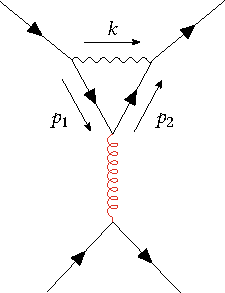
\includegraphics[width=\textwidth]{examples/feynman-diag.pdf}
\end{column}
\end{columns}
\end{frame}

\begin{frame}[fragile]
\frametitle{专业功能(三)}
\begin{itemize}
  \item 抄录:忽略所有特殊类别码\zhparen{catcode},原样显示

    \begin{itemize}
      \item |\verb<char>...<char>|、|verbatim| 环境
      \item \pkg{verbatim}、\pkg{fancyvrb} 宏包
    \end{itemize} \pause

  \item 语法高亮

    \begin{itemize}
      \item \pkg{listings} 宏包
      \item \pkg{minted} 宏包

        \begin{itemize}
          \item 需要 Python+Pygments,且开启 |--shell-escape|
          \item 也可尝试 Node.js+Shiki \link{https://github.com/shikijs/shiki-latex}
        \end{itemize}
    \end{itemize}
\end{itemize} \pause
\begin{lstlisting}[
  language         = C,
  xleftmargin      = 6em,
  numbers          = left,
  numberstyle      = \tiny,
  basicstyle       = \scriptsize\ttfamily,
  keywordstyle     = \color{emph1},
  commentstyle     = \itshape\color{comment},
  stringstyle      = \color{texcs},
  showstringspaces = false]
/* A standard Hello World program in C. */
#include <stdio.h>
int main(int argc, char** argv) {
    printf("Hello, world!\n");
    return 0;
}
\end{lstlisting}
\vspace{-1cm}
\end{frame}

\section{字体排印}

\begin{frame}{先看一个例子}
\begin{minipage}{\textwidth}
  \ArphicKai\small
  \hyphenpenalty=10000\hbadness=10000
  \linespread{0.8}\selectfont
  \textbf{Typography} is the art and technique of arranging type to make written language
  legible,readable,and appealing when displayed. The arrangement of type involves selecting
  typefaces, point sizes, line lengths, line-spacing(\textit{leading}), and letter-spacing
  (\textit{tracking}), and adjusting the space between pairs of letters(\textit{kerning}).
  The term typography is also applied to the style,arrangement, and appearance of the letters,
  numbers, and symbols created by the process. \textbf{Type design} is a closely related craft,
  sometimes considered part of typography;most typographers do not design typefaces, and some
  type designers do not consider themselves typographers. Typography also may be used as a
  decorative device,unrelated to communication of information.
\end{minipage}
\nonumberfootnote{文鼎楷体,行距 0.8 倍,关闭断词;
  文本来源:\link{https://en.wikipedia.org/wiki/Typography}}
\end{frame}

\begin{frame}{没有对比就没有伤害}
\begin{minipage}{\textwidth}
  \Garamond\small
  \textbf{Typography} is the art and technique of arranging type to make written language
  legible, readable, and appealing when displayed. The arrangement of type involves selecting
  typefaces, point sizes, line lengths, line-spacing (\textit{leading}), and letter-spacing
  (\textit{tracking}), and adjusting the space between pairs of letters (\textit{kerning}).
  The term typography is also applied to the style, arrangement, and appearance of the letters,
  numbers, and symbols created by the process. \textbf{Type design} is a closely related craft,
  sometimes considered part of typography; most typographers do not design typefaces, and some
  type designers do not consider themselves typographers. Typography also may be used as a
  decorative device, unrelated to communication of information.
\end{minipage}
\nonumberfootnote{EB Garamond,默认设置}
\end{frame}

\begin{frame}{术语}
\footnotesize
\begin{columns}[t]
\begin{column}{0.48\textwidth}
  \begin{itemize}
    \item 语言\zhparen{language}
    \item 文字\zhparen{script}
    \item 书写系统\zhparen{writting system}
    %
    \item 符号\zhparen{symbol}
    \item 字符\zhparen{character}
    \item 字符形\zhparen{glyph}
    %
    \item 字符集\zhparen{character set}
    \item 编码\zhparen{encoding}
    \item 码位\zhparen{code point}
  \end{itemize}
\end{column}
\begin{column}{0.48\textwidth}
  \begin{itemize}
    \item 字体\zhparen{font}
    \item 字型\zhparen{typeface}
    %
    \item 易认性\zhparen{legibility}
    \item 可读性\zhparen{readability}
    %
    \item 字偶间距\zhparen{kerning}
    \item 字距\zhparen{tracking}
    %
    \item 栅格化\zhparen{rasterization}
    \item 渲染提示\zhparen{hinting}
    \item ……
  \end{itemize}
\end{column}
\end{columns}
\end{frame}

\begin{frame}[standout]
  \large \textbf{\LaTeX{} will do (almost) all the things for you.}
\end{frame}

\begin{frame}[fragile]
\frametitle{Punctuations: hyphen/dash}
\begin{columns}
\begin{column}{0.84\textwidth}
  \begin{itemize}
    \item<1-> Hyphen \enparen{\usv{002D}}: |-|

      \begin{itemize}
        \item Four-dimensional momentum
        \item Hyphenation

          \begin{itemize}
            \item Hyphenation is language-dependent
            \item Use a dictionary to check breakable positions
          \end{itemize}
      \end{itemize}

    \item<3-> En dash \enparen{\usv{2013}}: |--|

      \begin{itemize}
        \item Ryu--Takayanagi formula (\textit{cf.} Levi-Civita symbol)
        \item pp.~187--189
      \end{itemize}

    \item<4-> Em dash \enparen{\usv{2014}}: |---|

      \begin{itemize}
        \item Red, white, and blue---these are the colors of the flag
        \item Like colon, parentheses, \textit{etc.}
      \end{itemize}

    \item<5-> Minus \enparen{\usv{2212}}: |$-$|

      \begin{itemize}
        \item $a-b$, $-a$
      \end{itemize}
  \end{itemize}
\end{column}
\begin{column}{0.13\textwidth}
  \onslide<2->
  \tiny\RaggedRight
  A hyphen\alert{-}ation algo\alert{-}rithm is a set of rules, especially one codified
  for imple\alert{-}mentation in a computer program, that decides at which points
  a word can be broken over two lines with a hyphen.
\end{column}
\end{columns}
\end{frame}

\begin{frame}[fragile]
\frametitle{Punctuations: quotation mark}
\begin{itemize}
  \item<1-> Left/right, single/double:

    \begin{itemize}
      \item `\ldots{}' \enparen{\usv{2018}, \usv{2019}}: |`...'|
      \item ``\ldots{}'' \enparen{\usv{201C}, \usv{201D}}: |``...''|
    \end{itemize}

  \item<2-> Different languages:

    \begin{itemize}
      \item `British ``English'' style' and ``American `English' style''
      \item „German'', ''Finnish'', «French», »Danish«, \textit{etc.}
      \item<3-> Use \pkg{csquotes} package
    \end{itemize}

  \item<4-> Programming:

    \begin{itemize}
      \item |char* my_name = "Xiangdong Zeng";|
    \end{itemize}

  \item<5-> Mathematics:

    \begin{itemize}
      \item |f'| = |f^{\prime}|: $f'(x) = f^{\prime}(x)$
    \end{itemize}
\end{itemize}
\end{frame}

\begin{frame}[fragile]
\frametitle{中文标点符号}
\begin{itemize}
  \item<+-> 句号

    \begin{itemize}
      \item 正常文本。科技文本.
    \end{itemize}

  \item<+-> 引号

    \begin{itemize}
      \item 『传统风格』,「某乎风格」,“标准风格”,\mbox{}’\kern-0.6em奇葩风格”
    \end{itemize}

  \item<+-> 破折号

    \begin{itemize}
      \item 断开\symbol{"2014}\symbol{"2014}是不好的,不断开——是好的
    \end{itemize}

  \item<+-> 波浪号:

    \begin{itemize}
      \item |~| ≠ |\textasciitilde| ≠ |\texttildelow| ≠ |$\sim$| ≠ 你要的那个
      \item 那就是~青\textasciitilde 藏\texttildelow 高 $\sim$ 原~~~~

        \begin{itemize}
          \item \texttt{\usv{007E}: Tilde}
          \item \texttt{\usv{02F7}: Modifier letter low tilde}
          \item \texttt{\usv{223C}: Tilde operator}
          \item \texttt{\usv{FF5E}: Fullwidth tilde}
          \item \ldots{}
        \end{itemize}
    \end{itemize}
\end{itemize}
\end{frame}

\begin{frame}{使用字体:\pkg{fontspec} 宏包}
\begin{itemize}
  \item<1-> 字体家族 \link{https://stone-zeng.github.io/2018-08-08-use-opentype-fonts}

    \begin{itemize}
      \item 衬线体:
        {\Garamond Garamond}, {\Times Times New Roman}, {\Bodini Bodini}, \textit{etc.}
      \item 无衬线体:
        {\Helvetica Helvetica}, {\Futura Futura}, {\Optima Optima}, \textit{etc.}
      \item 等宽字体:
        {\Courier Courier}, {\Inconsolata Inconsolata}, {\Unifont GNU Unifont}, \textit{etc.}
      \item 中文字体:
        宋体、{\heiti 黑体}、{\fangsong 仿宋}、{\kaishu 楷书}……
    \end{itemize}

  \item<2-> 样式 \link{https://stone-zeng.github.io/2019-07-06-use-opentype-fonts-ii}

    \begin{itemize}
      \item 粗体、意大利体:
        \textbf{Bold} vs {\addfontfeatures{AutoFakeBold=4}\textbf{Faked bold}},
        \textit{Italic} vs {\addfontfeatures{AutoFakeSlant=0.2}\textsl{Slant}}
      \item<3-> \alert{汉字一般不使用斜体}
      \item<4-> 视觉字号\zhparen{optical size}:\\
        {\LatinRomanV    Tiny},
        {\LatinRomanVI   Script},
        {\LatinRomanVII  Footnote},
        {\LatinRomanVIII Caption},
        {\LatinRomanIX   Small},
        {\LatinRomanX    Normal},
        {\LatinRomanXII  Large},
        {\LatinRomanXVII Huge}
    \end{itemize}

  \item<5-> OpenType 特性

    \begin{itemize}
      \item 连字\zhparen{ligature}:f{}f $\to$ ff, f{}i $\to$ fi, f{}l $\to$ fl
      \item 老式数字\zhparen{old-style number}:
        0123456789 $\to$ {\addfontfeatures{Numbers=OldStyle}0123456789}
      \item 字偶间距\zhparen{kerning}:T{}y $\to$ Ty, W{}A $\to$ WA
    \end{itemize}

  \item<6-> \alert{请避免滥用过多字体{\tiny (此页除外)}}
\end{itemize}
\vspace{-0.2cm}
\end{frame}

\section{进阶扩展}

\begin{frame}[fragile]
\frametitle{\TeX{} 宏编程}
\begin{itemize}
  \item<+-> \TeX{} 层面

    \begin{itemize}
      \item 守序善良——定义命令:|\def|、|\gdef|、|\let|
      \item 绝对中立——展开控制:|\edef|、|\expandafter|、|\aftergroup|
      \item 混乱邪恶——类别码:|\catcode|
    \end{itemize}

  \item<+-> \LaTeX{} 层面

    \begin{itemize}
      \item 定义新命令:|\newcommand|、|\renewcommand|、|\newenvironment|
      \item 内部命令:|\makeatletter|、|\makeatother|
    \end{itemize}

  \item<+-> \LaTeX3——可望还不可即的未来
    \link{https://github.com/xziyue/latex3-chinese-video}
    \link{https://stone-zeng.github.io/2019-02-24-l3tutorial-background}

    \begin{itemize}
      \item 命令举例:|\cs_new:cpx|、|\seq_sort:Nn|、|\regex_match:nnTF|
      \item 创建用户层命令:\pkg{xparse} 宏包(已默认载入)
      \item 面向对象编程、组件化:\pkg{xtemplate} 宏包
      \item \pkg{fontspec}、\pkg{siunitx}、\pkg{ctex}、\pkg{fduthesis} 等均使用 \LaTeX3 实现
      \item \LaTeX{} 内核正逐步迁移至 \LaTeX3
    \end{itemize}

  \item<+-> 外部语言调用

    \begin{itemize}
      \item |\write18|、|\directlua| 与 Python\TeX{}
    \end{itemize}
\end{itemize}
\end{frame}

\begin{frame}[fragile]
\frametitle{深入字体}
\begin{itemize}
  \item<+-> NFSS 与字体的坐标

    \begin{itemize}
      \item 字体族、形状、系列、编码、字号
      \item \TeX{} 仅需要 metric 信息:|.tfm|
    \end{itemize}

  \item<+-> 现代方案:OpenType

    \begin{itemize}
      \item 编码层面:支持 Unicode
      \item 东亚文字:超大字符集、地区变体、竖排
      \item 中东、南亚文字:Bi-di 文本、上下文连字、字符序调整
    \end{itemize}

  \item<+-> OpenType 中的数学支持(|MATH| 表)

    \begin{itemize}
      \item Unicode Math:字母、符号支持
      \item 「数学常数」:整体度量信息——上下标位置、分数线粗细等
      \item |MathVariants|:大小替换(积分号、根号、括号等)
      \item |MathGlyphConstruction|:字符形装配(更大的根号、括号等)
    \end{itemize}

  \item<+-> 可变字体\zhparen{
\includegraphics{examples/variable-font.pdf}}、
    \jatext{絵文字}\zhparen{emoji, \raisebox{-.2ex}{
\includegraphics{examples/emoji.pdf}}}……
\end{itemize}
\end{frame}

\begin{frame}[fragile]
\frametitle{编写宏包}
\begin{itemize}
  \item<+-> 文学编程

    \begin{itemize}
      \item 代码、注释与文档合为一体(|.dtx| 文件)
      \item 使用 \pkg{doc} 与 \pkg{docstrip} 宏包
      \item 但也增加了额外的复杂度
    \end{itemize}

  \item<+-> 发布

    \begin{itemize}
      \item 上传 CTAN 实际上并无门槛
      \item 但仍有必要了解:

        \begin{itemize}
          \item \TeX{} 目录结构(TDS)
          \item 测试系统:\pkg{l3build} 宏包
          \item 版本控制、持续集成
          \item 许可证选择:\LaTeX{} 内核使用 LPPL 1.3c
            \link{https://www.latex-project.org/lppl/lppl-1-3c}
        \end{itemize}
    \end{itemize}

  \item<+-> 参考

    \begin{itemize}
      \item \LaTeX{} 内核代码:\pkg{source2e.pdf}、\pkg{classes.pdf}、\pkg{source3.pdf}
      \item 书籍:\textit{The \TeX book}、\textit{\TeX{} by Topic}、\textit{The \LaTeX{} Companion} 等
    \end{itemize}
\end{itemize}
\end{frame}

\begin{frame}[fragile]
\frametitle{宏包推荐}
\footnotesize
\setbeamertemplate{itemize/enumerate subbody begin}{\scriptsize}
\setlength{\leftmarginii}{1.5em}
\begin{multicols}{3}
  \begin{itemize}
    \item 必备

      \begin{itemize}
        \item \pkg{amsmath}
        \item \pkg{graphicx}
        \item \pkg{hyperref}
      \end{itemize}

    \item 样式

      \begin{itemize}
        \item \pkg{caption}
        \item \pkg{enumitem}
        \item \pkg{fancyhdr}
        \item \pkg{footmisc}
        \item \pkg{geometry}
        \item \pkg{ntheorem}
        \item \pkg{titlesec}
      \end{itemize}

    \item 数学

      \begin{itemize}
        \item \pkg{bm}
        \item \pkg{mathtools}
        \item \pkg{physics}
        \item \pkg{unicode-math}
      \end{itemize}

    \item 表格

      \begin{itemize}
        \item \pkg{array}
        \item \pkg{booktabs}
        \item \pkg{longtable}
        \item \pkg{tabularx}
      \end{itemize}

    \item 插图、绘图

      \begin{itemize}
        \item \pkg{float}
        \item \pkg{pdfpages}
        \item \pkg{standalone}
        \item \pkg{subfig}
        \item \pkg{pgf}/\pkg{tikz}
        \item \pkg{pgfplots}
      \end{itemize}

    \item 字体

      \begin{itemize}
        \item \pkg{newtx}
        \item \pkg{newpx}
        \item \pkg{pifont}
        \item \pkg{fontspec}
      \end{itemize}

    \item 多语言

      \begin{itemize}
        \item \pkg{babel}
        \item \pkg{polyglossia}
        \item \pkg{ctex}
        \item \pkg{xeCJK}
        \item \pkg{luatexja}
      \end{itemize}

    \item 杂项功能

      \begin{itemize}
        \item \pkg{algorithm2e}
        \item \pkg{beamer}
        \item \pkg{biblatex}
        \item \pkg{fancyhdr}
        \item \pkg{listings}
        \item \pkg{mhchem}
        \item \pkg{microtype}
        \item \pkg{minted}
        \item \pkg{natbib}
        \item \pkg{siunitx}
        \item \pkg{xcolor}
      \end{itemize}
  \end{itemize}
\end{multicols}
\vspace*{-0.5cm}
\end{frame}

\begin{frame}[standout]
  \huge \textbf{请务必先读文档!} \\[1ex] \pause
  \footnotesize 命令行执行 \texttt{texdoc \textit{package}}
\end{frame}

\begin{frame}[fragile]
\frametitle[Markdown]{%
  Markdown \link{https://liam.page/2020/03/30/writing-manuscript-in-Markdown-and-typesetting-with-LaTeX}}
\begin{columns}
\lstset{%
  moredelim    = [s][emphstyle]{*}{*},
  moredelim    = [s][keywordstyle]{**}{**},
  moredelim    = [s][emphstyle2]{\`}{\`},
  moredelim    = [s][emphstyle2]{\`\`\`}{\`\`\`},
  moredelim    = [l][keywordstyle2]{\#},
  moredelim    = [is][keywordstyle2]{+}{+},
  moredelim    = *[is][\itshape]{!}{!},
  moredelim    = [is][keywordstyle]{(+}{+)},
  moredelim    = [is][emphstyle2]{(-}{-)},
  basicstyle   = \scriptsize\ttfamily,
  keywordstyle = [1]\bfseries\color{keyword},
  keywordstyle = [2]\bfseries\color{texcs},
  emphstyle    = [1]\itshape\color{emph1},
  emphstyle    = [2]\color{inline}}
\begin{column}{0.48\textwidth}
  \begin{lstlisting}[gobble=2]
  # Markdown syntax

  This is **bold text**.
  This text is *italicized*.
  Use `git status` to list all
  new or modified files.

  Block code:

  ```
  git status
  git add
  git commit
  ```

  Quotation:

  +>+ !Markdown uses email-style `>`!
  +>+ !characters for blockquoting.!
  \end{lstlisting}
\end{column}
\begin{column}{0.48\textwidth}
  \begin{lstlisting}[gobble=2]
  ## List

  ### Bullet list

  +*+ apples
  +*+ oranges
  +*+ pears

  ### Numbered list

  +1.+ wash
  +2.+ rinse
  +3.+ repeat

  +---+

  Link: from [(+Wikipedia+)]
  ((-https://en.wikipedia.org/wiki/-)
  (-Markdown-))

  \end{lstlisting}
\end{column}
\end{columns}
\vspace{-0.6cm}
\end{frame}

\begin{frame}[fragile]
\frametitle{Git}
\begin{itemize}
  \item<+-> 版本管理的必要性

    \begin{itemize}
      \item 远离「初稿,第二稿,第三稿……终稿,终稿(打死也不改了)」
      \item 有底气做大范围修改、重构
      \item 方便与他人协同合作
    \end{itemize}

  \item<+-> 基本用法

    \begin{itemize}
      \item 把大象放进冰箱:|git init|、|git add|、|git commit|
      \item 时空穿梭:|git reset|、|git revert|
      \item 平行宇宙:|git branch|、|git checkout|、|git rebase|
      \item 推荐用 VS Code 等进行可视化操作
      \item 参考链接:\link{https://git-scm.com/book}
        \link{https://www.liaoxuefeng.com/wiki/0013739516305929606dd18361248578c67b8067c8c017b000}
    \end{itemize}

  \item<+-> GitHub \href{https://github.com}{\faGithub}

    \begin{itemize}
      \item 远程 Git 仓库
      \item Clone \& fork
      \item Issues \& pull requests
      \item<+-> \alert{提醒:绑定 \texttt{.edu} 邮箱可以有更多优惠}
    \end{itemize}
\end{itemize}
\end{frame}

\begin{frame}{获取帮助}
\begin{itemize}
  \item<+-> 搜索、提问的姿势

    \begin{itemize}
      \item 优先使用英文 + Google (if possible)
      \item 提供最小工作示例(MWE, minimal working example)
        \begin{itemize}
          \item 能复现问题
          \item 尽量不带冗余内容
          \item 策略:二分查找
        \end{itemize}
      \item 遵循社区行为准则(code of conduct)
    \end{itemize}

  \item<+-> 在线论坛

    \begin{itemize}
      \item \TeX{} - \LaTeX{} Stack Exchange \link{https://tex.stackexchange.com}
      \item \CTeX{} 临时论坛 \link{https://github.com/CTeX-org/forum}
      \item \LaTeX{} 工作室 \link{https://www.latexstudio.net}
        \begin{itemize}
          \item 资源需要甄别,且部分内容需付费
        \end{itemize}
    \end{itemize}
\end{itemize}
\end{frame}

\begin{frame}{社区参与}
\begin{itemize}
  \item 文档翻译

    \begin{itemize}
      \item \pkg{lshort-zh-cn} \link{https://github.com/CTeX-org/lshort-zh-cn}
      \item \pkg{learnlatex.org/zh} \link{https://github.com/CTeX-org/learnlatex.github.io}
    \end{itemize}

  \item 宏包开发与维护

    \begin{itemize}
      \item 不妨先从修 typo 开始
      \item 参与讨论,你的经验也可以解他人之忧
        \link{https://github.com/stone-zeng/fduthesis/discussions}
        \link{https://github.com/tuna/thuthesis/discussions}
        \link{https://github.com/sjtug/SJTUThesis/discussions}
      \item 欢迎参与维护 \pkg{fdutheis}
    \end{itemize}

  \item \CJKsout{来当主讲人}
\end{itemize}
\end{frame}

\begin{frame}[fragile]
\frametitle{参考文献与扩展阅读}
\begin{multicols}{2}
\tiny
\newcommand{\BOOK}[1]{\textbf{#1}}
\newcommand{\TAG}[1]{\CASE{[#1]}}
\newcommand{\URL}[1]{\scalebox{0.92}[1]{\url{#1}}}
\begin{thebibliography}{99}
  \bibitem{}
    \textsc{Knuth D E}.
    \BOOK{The \TeX book: Computers \& Typesetting, volume C} \TAG{M}, 1984.
    \newblock Addison--Wesley Publishing Company, Boston
  \bibitem{}
    \textsc{Bringhurst R}.
    \BOOK{The Elements of Typographic Style, version 4.3} \TAG{M}, 2019.
    \newblock Hartley \& Marks Publishers, Vancouver
  \bibitem{}
    刘海洋.
    \BOOK{\LaTeX{} 入门} \TAG{M}, 2013.
    \newblock 北京:电子工业出版社
  \bibitem{}
    \jatext{高冈昌生}.
    刘庆~译,陈嵘~监修.
    \BOOK{西文排版:排版的基础和规范} \TAG{M}, 2016.
    \newblock 北京:中信出版集团
  \bibitem{}
    \textsc{Oetiker T}, \textsc{Partl H}, \textsc{Hyna I} and \textsc{Schlegl E}.
    \CTeX{} 开发小组~译.
    \BOOK{一份(不太)简短的 \LaTeXe{} 介绍:或 111 分钟了解 \LaTeXe{}} \TAG{EB/OL}, 2021.
    \newblock \URL{https://ctan.org/pkg/lshort-zh-cn}
  \bibitem{}
    黄新刚(包太雷).
    \BOOK{\LaTeX{} Notes: 雷太赫排版系统简介(第二版)} \TAG{EB/OL}, 2021.
    \newblock \URL{https://github.com/huangxg/lnotes}
  \bibitem{}
    汪彧之,陈晟祺.
    \BOOK{清华大学图书馆:如何使用 \LaTeX{} 排版论文} \TAG{EB/OL}, 2021.
    \newblock \URL{https://github.com/tuna/thulib-latex-talk}
  \bibitem{}
    吴伟健,李子龙.
    \BOOK{上海交通大学图书馆:如何使用 \LaTeX{} 排版论文} \TAG{EB/OL}, 2022.
    \newblock \URL{https://github.com/sjtug/sjtulib-latex-talk}
  \bibitem{}
    刘海洋.
    \BOOK{\LaTeX{} \CJKsout[thickness=0.1em]{快速}入门} \TAG{EB/OL}, 2020.
    \newblock Video: \href{https://www.bilibili.com/video/BV1s7411U7Pr}{\faVideo}
    % Old version: https://bbs.pku.edu.cn/attach/e7/f2/e7f2bb698b9c3672/tex_intro_talk.pdf
  \bibitem{}
    林莲枝.
    \BOOK{漫谈 \LaTeX{} 排版常见概念误区:别把 \LaTeX{} 当 Word 用!}\TAG{EB/OL}, 2018.
    \newblock Video: \href{https://www.bilibili.com/video/BV1r4411o7KJ}{\faVideo}\quad
      PDF: \href{http://static.latexstudio.net/wp-content/uploads/2018/03/LianTze-presentation-0320-forReading.pdf}{\faDownload}
  \bibitem{}
    Wikibooks.
    \BOOK{\LaTeX{}---Wikibooks, The Free Textbook Project} \TAG{EB/OL}.
    \newblock \URL{https://en.wikibooks.org/wiki/LaTeX}
  \bibitem{}
    Overleaf.
    \BOOK{Overleaf Documentation} \TAG{EB/OL}.
    \newblock \URL{https://www.overleaf.com/learn}
  \bibitem{}
    \LaTeX{} project.
    \BOOK{Learn\LaTeX.org} \TAG{EB/OL}.
    \newblock \URL{https://www.learnlatex.org}
\end{thebibliography}
\end{multicols}
\end{frame}

\begin{frame}{关于}
\vspace*{1.2cm}
\footnotesize
本幻灯片:\url{https://github.com/stone-zeng/latex-talk} \\
最后更新:\DTMnow \\
许可证:Creative Commons Attribution-ShareAlike 4.0 International
\vspace{0.4cm}
\begin{center}
  \huge
  \faCreativeCommons\,\faCreativeCommonsBy\,\faCreativeCommonsSa
\end{center}
\vspace{2cm}
\begin{flushleft}
  \tiny
  Beamer 主题:萧山 \link{https://ctan.org/pkg/pgfornament-han} \\
  正文字体:思源宋体 + Libertinus Serif \\
  等宽字体:思源黑体 + Roboto Mono
\end{flushleft}
\vspace{-0.5cm}
\end{frame}

\begin{frame}[standout]
  \huge \textbf{\texttt{\textbackslash bye}}
\end{frame}


\end{document}
